\chapter{String Theory and M-Theory}

Susskind opens by promising a ``space-time view'' of string theory and then immediately backs up to something simpler: an ordinary particle. That retreat is not a detour. It is the structure of the lecture. We first learn how to think about a trajectory, an action, and a sum over histories in the familiar one-dimensional setting; only then do we lift the same logic to a string and its worldsheet. These companion notes follow Leonard Susskind's Lecture~7, with supporting blackboard evidence curated from the video by LazyingArt LLC and Video2Book.

\section{From Particle Trajectories to Path Integrals}

Let us begin exactly where the lecture begins: with an ordinary particle. In nonrelativistic mechanics we describe its motion by a trajectory \(x(t)\), and for a free particle with mass set equal to~\(1\) the action is
\begin{equation}
S_{\mathrm{NR}}=\int dt\,\frac12 \dot{x}^{\,2}.
\end{equation}
In relativistic mechanics the more natural description is to package space and time together into \(X^\mu\), and to regard \(X^\mu\) as a function of a scalar parameter \(\tau\) along the trajectory. In the lecture \(\tau\) is taken to be proper time. The relativistic action is then written schematically as
\begin{equation}
S_{\mathrm{rel}}\sim \int d\tau\,\frac{dX^\mu}{d\tau}\frac{dX_\mu}{d\tau},
\end{equation}
with the contraction between the upper and lower indices understood.

Up to that point the story is classical. We hold the endpoints fixed and minimize the action. In either case the free solution is the same in spirit: a straight line in spacetime, traversed with constant velocity. But now the lecture makes its first important turn. In quantum mechanics we do not ask, ``Which path is taken?'' We ask, ``What is the amplitude to go from here to there?''

To a given path we attach a phase. In the nonrelativistic case that phase is
\begin{equation}
\exp\!\left(i\int_{t_1}^{t_2} dt\,\frac12 \dot{x}^{\,2}\right).
\end{equation}
Then we do not stop with one path. We integrate over all paths connecting the two endpoints:
\begin{equation}
K(1\to 2)=\int \mathcal{D}x\,e^{iS[x]}.
\end{equation}
That is the Feynman path integral. In relativistic language the amplitude to go from one spacetime point to another is the propagator. More elaborate processes are built by joining segments, summing the actions for the segments, integrating over the joining points, and finally summing over diagrams. In that sense the path integral is already the seed from which the whole diagrammatic expansion grows.

The important conceptual move, and Susskind insists on it, is this: the action is still central, but it is no longer something we simply minimize. It is something we exponentiate and sum over.

\section{The Physicist's Cheat: Turning Time Sideways}

Before going to strings, the lecture stops to confront a technical problem that would otherwise be swept under the rug. The formal path integral is a monstrosity. Every trajectory contributes a factor of magnitude one, because \(|e^{iS}|=1\). The tame trajectories and the wild ones differ only by phase.

That already tells us why classical motion is not obvious from the integral. The nearly classical paths must emerge only after enormous cancellations among wildly oscillating contributions. This may be physically right, but it is not a friendly way to define an integral.

\subsection{Question \& Answer}

\paragraph{Question.} Why does Wick rotation make the path integral manageable without changing the physics we want in the end?

\paragraph{Answer.} Because it turns a purely oscillatory weight into a decaying one. Wild trajectories, which were previously unsuppressed in magnitude, acquire a large positive Euclidean action and are exponentially damped. One first computes the convergent Euclidean object and then analytically continues back to the physical domain.

Susskind illustrates the trick in the relativistic particle notation. Introduce a new parameter \(s\) by
\begin{equation}
\tau=\alpha s.
\end{equation}
He jokes about the collision between this little \(s\), the action, and the Mandelstam variable that will appear later; for the notes we keep \(S\) for the action and use \(s\) only locally in this calculation. With
\begin{equation}
d\tau=\alpha\,ds,
\qquad
\frac{dX}{d\tau}=\frac{1}{\alpha}\frac{dX}{ds},
\end{equation}
the quadratic action becomes
\begin{equation}
\int d\tau\,\left(\frac{dX}{d\tau}\right)^2
=
\frac{1}{\alpha}\int ds\,\left(\frac{dX}{ds}\right)^2.
\end{equation}
Now choose \(\alpha=-i\). Then the \(i\) in the phase combines with the \(1/\alpha\) to produce a minus sign, and the path weight takes the Euclidean form
\begin{equation}
e^{iS}
\longrightarrow
\exp\!\left[-\frac12\int ds\,\left(\frac{dX}{ds}\right)^2\right].
\end{equation}
This is the stabilized version of the lecture's live blackboard derivation. A trajectory that shoots far away and comes back, or one that wiggles rapidly, makes \(\frac{dX}{ds}\) large; the Euclidean action is then large and positive, and the exponential is small.

That is the basic point. In this form the integral becomes a Wiener-type integral, the kind of object mathematicians know how to define seriously. The price is that we have changed the time variable into an imaginary one. The way back is analytic continuation. Susskind says, only half joking, that this is how physicists actually do path integrals: first turn time on its side, then continue back at the end.

\section{From Worldlines to Worldsheets}

With that trick in hand, we move to strings. The lecture says: same kind of setup, but now the particle is not a point. Its history is not a worldline. It is a surface. For an open string that surface is ribbon-like; for a closed string it is tube-like. In either case we introduce two coordinates on the worldsheet, \(\sigma\) and \(\tau\), and write
\begin{equation}
X^\mu=X^\mu(\sigma,\tau).
\end{equation}
These are not spacetime coordinates. They are parameters labeling points on the sheet. If we know \(X^\mu(\sigma,\tau)\) for every \((\sigma,\tau)\), then we know the whole history of the string in spacetime.

The action is the immediate two-variable analog of the particle action. The blackboard frame secures the derivative structure and the relative sign, though not the full normalization. We therefore write the action in the cautious standard form
\begin{equation}
S_{\mathrm{ws}}
\propto
\int d\tau\,d\sigma
\left[
\left(\partial_\tau X^\mu\right)^2
-
\left(\partial_\sigma X^\mu\right)^2
\right].
\end{equation}
The \(\tau\)-derivative term plays the role of kinetic energy; the \(\sigma\)-derivative term plays the role of potential energy. The minus sign is simply the worldsheet version of \(T-V\).

\begin{figure}
\centering

\includegraphics[width=0.62\textwidth]{lecture_07_figure_02.png}
\caption{Blackboard evidence for the worldsheet action density: a \(\tau\)-derivative term opposed by a \(\sigma\)-derivative term. The full coefficient and measure are not fixed by the frame alone.}
\end{figure}

Quantum mechanically we exponentiate and sum over all surfaces:
\begin{equation}
\mathcal{A}
=
\int \mathcal{D}X\,e^{iS_{\mathrm{ws}}[X]}.
\end{equation}
This is the amplitude for the string to go from a prescribed initial configuration to a prescribed final configuration. For a moment Susskind almost calls this the definition of string theory, and then immediately corrects himself: it is too simple. One must also allow processes in which two strings become three, or two become two, and one must sum over the surfaces interpolating between those boundary conditions. If holes are included, one has the analog of summing over all loop topologies in ordinary quantum field theory.

The lecture also pauses for a useful bridge back to familiar physics. A student asks whether, in a point-particle limit, one somehow simply ``sets \(\sigma\) to zero.'' Susskind's answer is more sensible than that: before string theory there is no \(\sigma\) at all, but in the low-energy regime string amplitudes do reproduce ordinary Feynman diagrams. So the two pictures are not disconnected. The string path integral is broader, but it contains the point-particle expansion in the appropriate limit.

\begin{remark}
Susskind briefly points to a more geometric action principle: proper length for a particle, and spacetime area for a string. In later language the string version is the Nambu--Goto action. He also mentions the Polyakov and Liouville names in passing. The lecture does not use those formalisms here; the point of the aside is historical and geometric, not part of the main derivation.
\end{remark}

\section{Euclidean Equation of Motion and the Laplace Form}

At this point the lecture changes register. The string path integral has been written down, and now Susskind says he wants to explain some mathematics. The motivating question is very concrete: what freedom do we really have in the choice of \((\sigma,\tau)\)? He never told us how to choose those coordinates on the worldsheet in the first place. They are only labels of points. One could call them George, Fred, and Harvey if one liked; the physics should not depend on that choice. So the real question is: under what changes of worldsheet coordinates is the theory invariant?

Instead of staring directly at the action, he turns to the equation of motion. That is not a different problem. It is just an easier way to see the invariant content. In Lorentzian form the action would lead to the ordinary wave equation
\begin{equation}
\partial_\tau^2 X-\partial_\sigma^2 X=0.
\end{equation}
But the lecture is now working in the Euclideanized setting. After the Wick rotation of the worldsheet time variable, the action can be written schematically as
\begin{equation}
S_{E,\mathrm{ws}}
\propto
\int d\tau\,d\sigma
\left[
\left(\partial_\tau X^\mu\right)^2
+
\left(\partial_\sigma X^\mu\right)^2
\right],
\qquad
\mathcal{A}\sim \int \mathcal{D}X\,e^{-S_{E,\mathrm{ws}}}.
\end{equation}
The lecture sorts out the signs live on the board, correcting itself more than once; the stable conclusion is that both terms become positive in the Euclidean action, so wildly stretched or violently vibrating surfaces are suppressed.

Now vary the action. First derivatives in the action produce second derivatives in the equation of motion, just as \(\dot{x}^{\,2}\) produces \(\ddot{x}\) in the particle problem. For one component \(X\) of the embedding field, the Euclidean equation is
\begin{equation}
\frac{\partial^2 X}{\partial \tau^2}+\frac{\partial^2 X}{\partial \sigma^2}=0.
\end{equation}
This is the two-dimensional Laplace equation.

\subsection{Question \& Answer}

\paragraph{Question.} Why does the board now show a plus-sign Laplace equation instead of the usual wave equation with a minus sign?

\paragraph{Answer.} Because the lecture has already performed the Wick-rotation trick on the worldsheet time variable. Before that step the classical equation is the Lorentzian wave equation \(\partial_\tau^2 X-\partial_\sigma^2 X=0\). After Euclideanization, the relative sign changes, and the equation takes the Laplace form \(\partial_\tau^2 X+\partial_\sigma^2 X=0\).

\begin{figure}
\centering

\includegraphics[width=0.64\textwidth]{lecture_07_figure_03.png}
\caption{The plus-sign equation as it appears on the board, together with the first discrete geometric sketch below it.}
\end{figure}

\begin{figure}
\centering
\begin{tikzpicture}[scale=1]
\draw (-4,0) -- (4,0);
\foreach \x in {-3.7,-3.3,-2.9,-2.5,-2.1,-1.7,-1.3,-0.9,-0.5,-0.1,0.3,0.7,1.1,1.5,1.9,2.3,2.7,3.1,3.5}
  \draw (\x,-0.08) -- (\x,0.08);
\end{tikzpicture}
\caption{A clean redraw of the discretized line that begins the geometric interpretation of the second derivative.}
\end{figure}

The lecture now deliberately slows down. Rather than announcing conformal invariance at once, Susskind asks a simpler question: what does this equation actually mean?

\section{Discrete Derivatives and the Average-Value Property}

To answer that question, the lecture turns the differential equation into a discrete one. First think of a single axis, divided into neighboring points \(1\), \(2\), and \(3\), with spacing \(\epsilon\). The exact factors of \(\epsilon\) are not the point here; the geometric structure is the point.

A first derivative is represented by a first difference, for example \(X(3)-X(2)\). So a second derivative is the difference of two neighboring first differences:
\begin{align}
\partial^2 X
&\leadsto
\bigl[X(3)-X(2)\bigr]-\bigl[X(2)-X(1)\bigr] \\
&=
X(3)+X(1)-2X(2).
\end{align}
This is precisely the algebra visible on the board, up to the fact that the rightmost bracket is partly cut off in the frame and must be completed from the lecture's spoken derivation.

\begin{figure}
\centering

\includegraphics[width=0.72\textwidth]{lecture_07_figure_04.png}
\caption{The finite-difference development on the blackboard: the same Laplace-form equation, a numbered discrete line, a small lattice sketch, and the simplified second-difference formula.}
\end{figure}

\begin{figure}
\centering
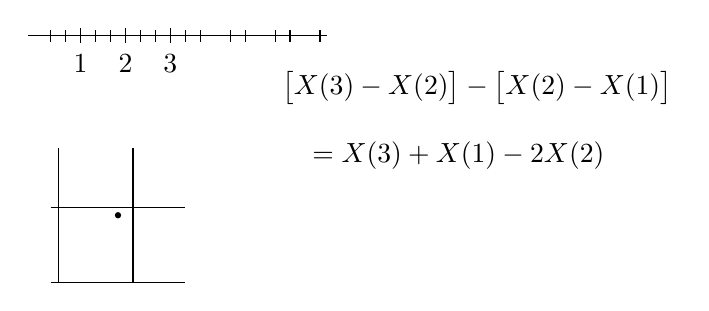
\begin{tikzpicture}[scale=0.95]
\draw (-4.4,2.3) -- (-0.4,2.3);
\foreach \x/\lab in {-3.7/1,-3.1/2,-2.5/3}
{
  \draw (\x,2.2) -- (\x,2.4);
  \node[below] at (\x,2.18) {\(\lab\)};
}
\foreach \x in {-4.1,-3.9,-3.5,-3.3,-2.9,-2.7,-2.3,-2.1,-1.7,-1.5,-1.1,-0.9,-0.5}
  \draw (\x,2.22) -- (\x,2.38);

\draw (-4.1,0.8) grid (-2.3,-1.0);
\fill (-3.2,-0.1) circle (1.2pt);

\node at (1.6,1.6) {\(\bigl[X(3)-X(2)\bigr]-\bigl[X(2)-X(1)\bigr]\)};
\node at (1.35,0.7) {\(=X(3)+X(1)-2X(2)\)};
\end{tikzpicture}
\caption{A clean redraw of the one-dimensional finite-difference argument and the small lattice patch that prepares the two-dimensional Laplacian.}
\end{figure}

Now discretize the full \((\sigma,\tau)\)-plane. Take a small square of neighboring points around a center, and label them \(1,2,3,4\) with the center labeled \(5\). In the lecture's board orientation, \(\tau\) happens to run horizontally and \(\sigma\) vertically; that is only a choice of labels. Then
\begin{equation}
\partial_\tau^2 X \leadsto X(1)+X(3)-2X(5),
\qquad
\partial_\sigma^2 X \leadsto X(2)+X(4)-2X(5).
\end{equation}
Adding them, because the Euclidean equation has a plus sign, we get
\begin{align}
0
&=
\bigl[X(1)+X(3)-2X(5)\bigr]
+
\bigl[X(2)+X(4)-2X(5)\bigr] \\
&=
X(1)+X(2)+X(3)+X(4)-4X(5).
\end{align}
So the Laplace equation may be rewritten as
\begin{equation}
X(5)=\frac14\bigl[X(1)+X(2)+X(3)+X(4)\bigr].
\end{equation}

\subsection{Question \& Answer}

\paragraph{Question.} What does the Laplace equation mean geometrically at a point?

\paragraph{Answer.} It means that at the center of an infinitesimal square, the field equals the average of the values at the corners. That is the local geometric content of the equation. The square may be rotated; the statement is invariant under rotations of the \((\sigma,\tau)\)-plane.

This is the decisive interpretive step of the lecture. The PDE is no longer an abstraction. It has become an averaging rule.

\section{Conformal Invariance of the Worldsheet}

Now the symmetry becomes almost obvious. If the equation says that the field at the center of every infinitesimal square is the average of the field at the corners, then the allowed coordinate transformations must be those that preserve infinitesimal squares. That is Susskind's first formulation of the invariance.

He then restates the same idea in the more standard language of angles. A transformation that preserves angles takes infinitesimal squares to infinitesimal squares, though it may change their size by a local scale factor. So the relevant symmetry is conformal symmetry.

The lecture is careful not to let this become a slogan too quickly. Conformal maps preserve local shape, not global size. A tiny square may map to a larger or smaller tiny square. Different regions of the plane may be expanded or contracted by different amounts. And for finite regions with boundaries, the corners of a square need not map to the corners of the image region. That is why one may conformally map a region with a simple boundary to a region with a very different-looking boundary shape without contradicting local angle preservation.

There is a brief side excursion to ordinary map projections. The point is not geography. It is that there are familiar maps which preserve the local shapes of islands and continents while distorting their sizes. That is exactly the sort of transformation under discussion here. The lecture also remarks, without developing the machinery, that coordinate transformations defined by analytic functions of a complex variable are angle-preserving. This is the mathematical doorway through which the next part of the lecture walks.

\section{From the Band-Aid to the Disc and Back to Duality}

Having built the local mathematics, the lecture now returns to last week's string-scattering geometry. Two strings come in, join to form one string, propagate for a while, and then split again. Susskind draws this as a slit ribbon, jokingly renamed the infinite sports band-aid. There is a one-parameter family of such worldsheets, characterized by the \(\tau\)-interval between the joining and splitting points. In the end one integrates over that parameter, and that integral is what gave the Euler beta function, or Veneziano amplitude.

Now comes the payoff of conformal invariance. After Euclideanization, the worldsheet fields satisfy the Laplace equation, and the Laplace equation is conformally invariant. Therefore the awkward slit-strip worldsheet may be mapped to a disc without changing the form of the equations in the interior. The embedding fields \(X^\mu\) may be regarded just as well as living on the disc.

There are, however, four special points on the boundary. They are the images of the four asymptotic external string states. The lecture does not yet build the formalism in detail, but it says clearly what later language will call the answer: one places vertex operators at those special points. Susskind temporarily calls them the injection points.

\subsection{Question \& Answer}

\paragraph{Question.} Why do four boundary insertion points leave only one real parameter, and how does that single modulus reproduce both the long-time direct channel and the crossed channel?

\paragraph{Answer.} Because conformal transformations of the disc still allow us to move the boundary points around. After using that freedom to choose a convenient left-right and up-down symmetric representative, only one genuine parameter remains. That surviving modulus is the disc-language image of the old joining--splitting interval on the slit worldsheet. Its two extreme limits correspond to two different channel pictures: a long-lived intermediate string in one limit, and the crossed-channel configuration in the other.

A symmetric schematic disc picture is therefore enough to capture the essential geometry:

\begin{figure}
\centering
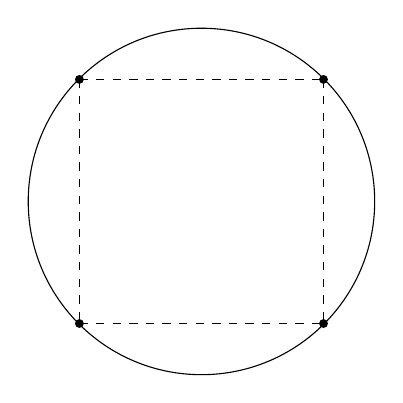
\begin{tikzpicture}[scale=1.0]
\draw (0,0) circle (2.2);
\fill (-1.55,1.55) circle (1.6pt);
\fill (1.55,1.55) circle (1.6pt);
\fill (-1.55,-1.55) circle (1.6pt);
\fill (1.55,-1.55) circle (1.6pt);
\draw[dashed] (-1.55,1.55) -- (1.55,1.55);
\draw[dashed] (-1.55,-1.55) -- (1.55,-1.55);
\draw[dashed] (-1.55,1.55) -- (-1.55,-1.55);
\draw[dashed] (1.55,1.55) -- (1.55,-1.55);
\end{tikzpicture}
\caption{A schematic disc with four special boundary points. The stable content from the lecture is that, modulo conformal symmetry, their configuration depends on only one real parameter.}
\end{figure}

The lecture emphasizes that the integral over the old joining--splitting time has not disappeared. It has merely been translated into an integral over the positions of these boundary insertion points, restricted to a one-parameter family after conformal redundancy is removed. In this language the beta function comes from integrating over that one remaining parameter.

The two extreme limits of the parameter correspond to two extreme boundary configurations. In one limit the two incoming points are close together, and this corresponds to the band-aid geometry in which the intermediate string lives for a very long time before splitting. In the other limit a different pair of points comes close together, corresponding to the crossed-channel picture.

The board sketches at the end of the lecture are valuable precisely because they make this symmetry visible.

\begin{figure}
\centering

\includegraphics[width=0.56\textwidth]{lecture_07_figure_06.png}
\caption{The paired end-of-lecture sketches that exhibit the symmetry between the two extreme channel pictures.}
\end{figure}

\begin{figure}
\centering
\begin{tikzpicture}[scale=0.95]
\draw (-3,1.8) -- (-1.0,0.3);
\draw (-3,4.6) -- (-1.0,3.1);
\draw (3,1.8) -- (1.0,0.3);
\draw (3,4.6) -- (1.0,3.1);
\draw (-1.0,3.1) -- (-0.5,3.35);
\draw (-0.5,3.35) -- (0.0,3.1);
\draw (0.0,3.1) -- (0.5,3.35);
\draw (0.5,3.35) -- (1.0,3.1);

\draw (-3,-4.6) -- (-1.0,-3.1);
\draw (-3,-1.8) -- (-1.0,-0.3);
\draw (3,-4.6) -- (1.0,-3.1);
\draw (3,-1.8) -- (1.0,-0.3);
\draw (-1.0,-3.1) -- (0.0,-3.1);
\draw (1.0,-3.1) -- (0.25,-3.1);
\draw (-1.0,-0.3) -- (0.0,-0.9);
\draw (1.0,-0.3) -- (0.25,-0.9);
\draw (0.0,-3.1) -- (0.25,-2.55);
\draw (0.25,-2.55) -- (0.0,-2.0);
\draw (0.0,-2.0) -- (0.25,-1.45);
\draw (0.25,-1.45) -- (0.0,-0.9);
\end{tikzpicture}
\caption{A clean redraw of the paired interaction sketches. The point is the geometric comparison between the two limits, not a detailed assignment of labels.}
\end{figure}

At the end of the lecture the channel language becomes stable again. In the all-incoming convention one has
\begin{equation}
s=(k_1+k_2)^2,
\qquad
t=(k_1+k_3)^2.
\end{equation}
The direct-channel picture is the one in which \(k_1\) and \(k_2\) effectively come together to form the intermediate state; the crossed-channel picture is the one in which \(k_1\) and \(k_3\) are paired instead. The remarkable claim is that one and the same integral accounts for both. What once looked like a miracle in the band-aid picture becomes structurally natural on the conformally mapped disc: the four-point amplitude is symmetric under interchange of the two channels,
\begin{equation}
\mathcal{A}_4(s,t)=\mathcal{A}_4(t,s).
\end{equation}
This is the original \(s\)-\(t\) channel duality.

\section{Summary}

The lecture begins with the particle so that the logic of string theory will not look mysterious when it arrives. First comes the classical action, then the quantum amplitude, then the realization that the oscillatory path integral is too wild to handle directly, and finally the Wick-rotation trick that turns it into a convergent Euclidean object.

Once the same structure is lifted from worldlines to worldsheets, the question of worldsheet coordinate freedom becomes unavoidable. In the Euclideanized setting the equation of motion is the Laplace equation. Interpreted discretely, that equation says that the value at the center of an infinitesimal square is the average of the values at the corners. From that local geometric fact, conformal invariance follows naturally: the allowed coordinate changes are precisely those that preserve infinitesimal squares, or equivalently angles.

The last step is the real payoff. Conformal invariance lets us replace the awkward slit-strip scattering surface by the disc with four special boundary points. The remaining one-parameter family of boundary configurations is the disc-language image of the old joining--splitting interval, and its two extreme limits are the direct and crossed channel pictures. The lecture ends by showing that these are not two unrelated processes at all, but two limits of one integral. That is the mathematical content of channel duality, and it is the point at which the geometry of the worldsheet begins to explain what had once looked miraculous.